\ESKDappendix{рекомендуемое}{Получение и использование математической модели плоского двухзвенного манипулятора}\label{app_examples}
Для пояснения описанных в документе действий составим и подробно распишем математическую модель плоского двухзвенного манипулятора, показанного на рисунке~\ref{img_manipulator_2}.

\begin{figure}[h!]
    \begin{minipage}[h]{0.5\linewidth}
        \centering{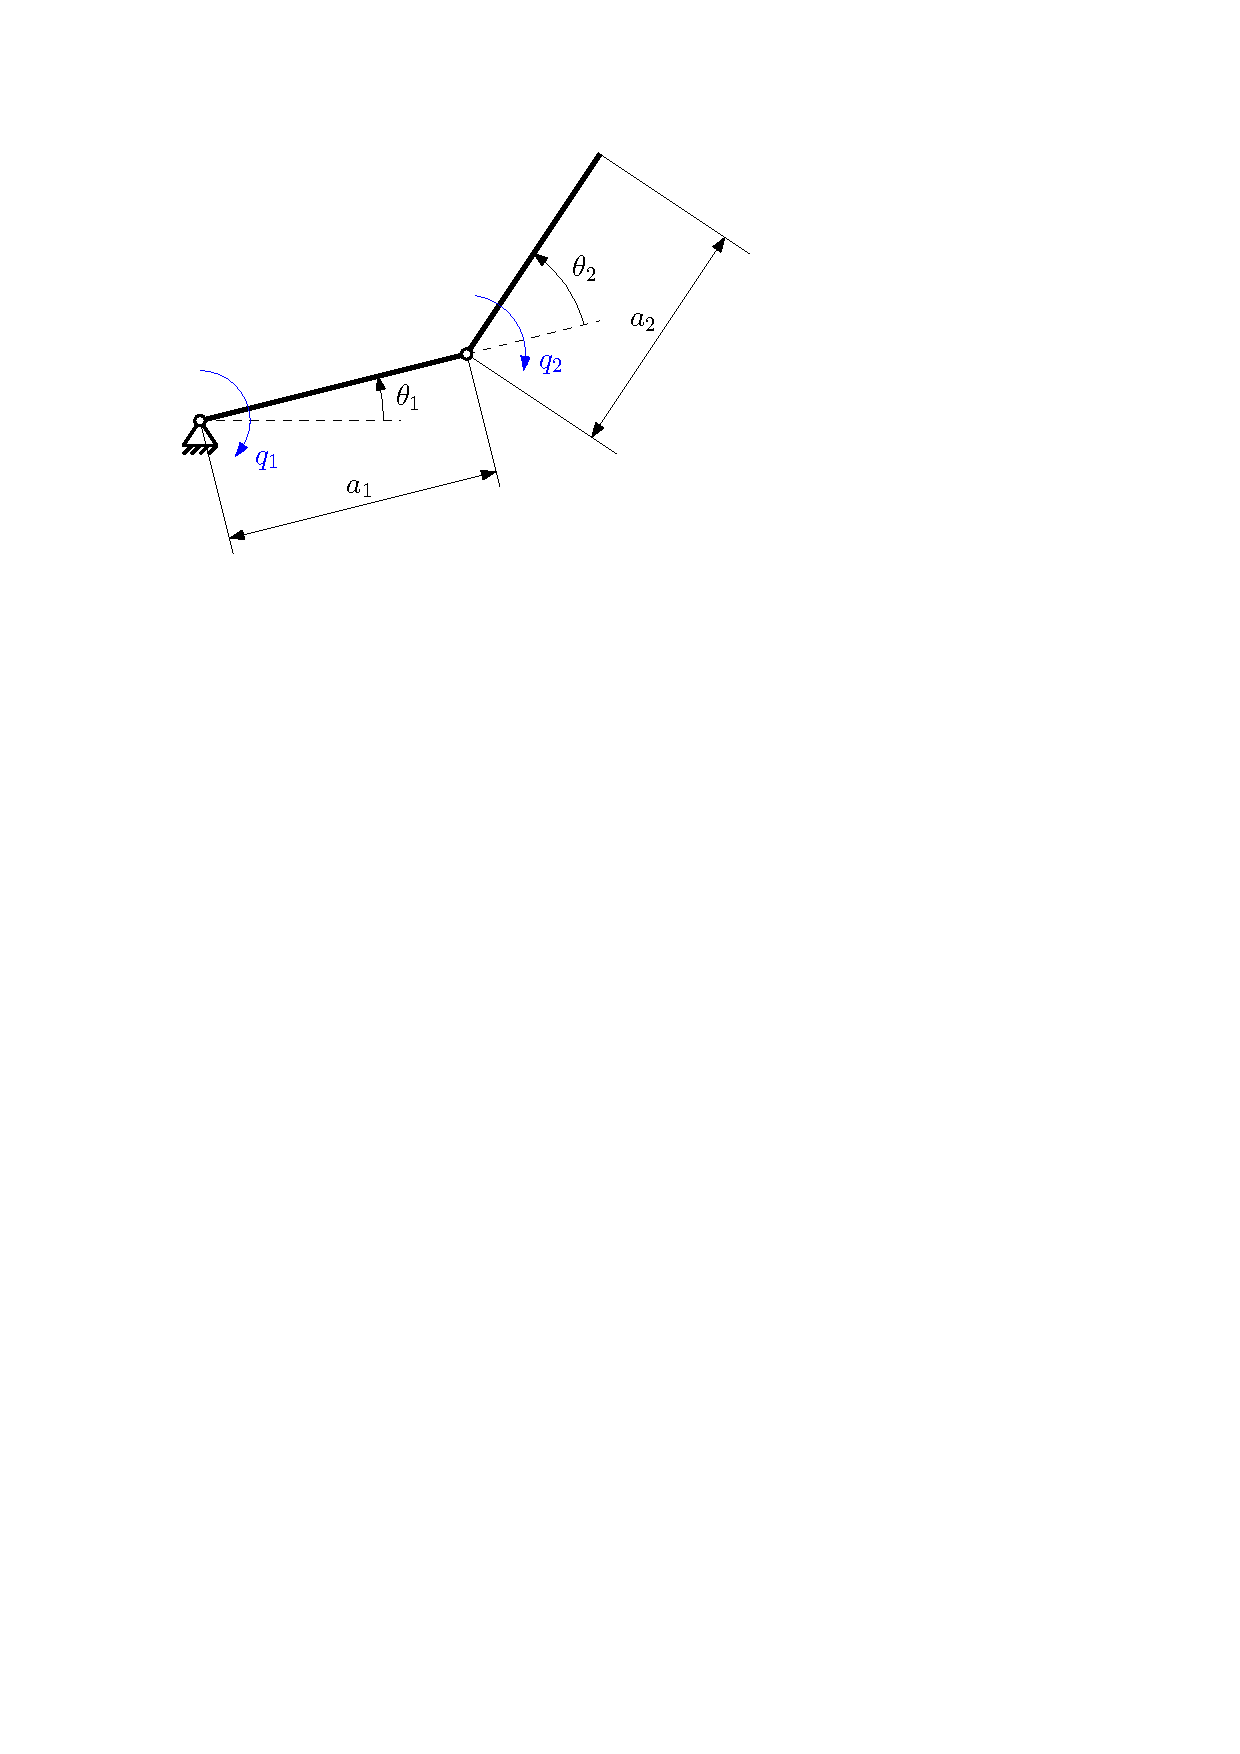
\includegraphics[width=0.95\linewidth]{manipulator_2_kinematics.pdf} \\ а)}
    \end{minipage}
    \hfill
    \begin{minipage}[h]{0.5\linewidth}
         \centering{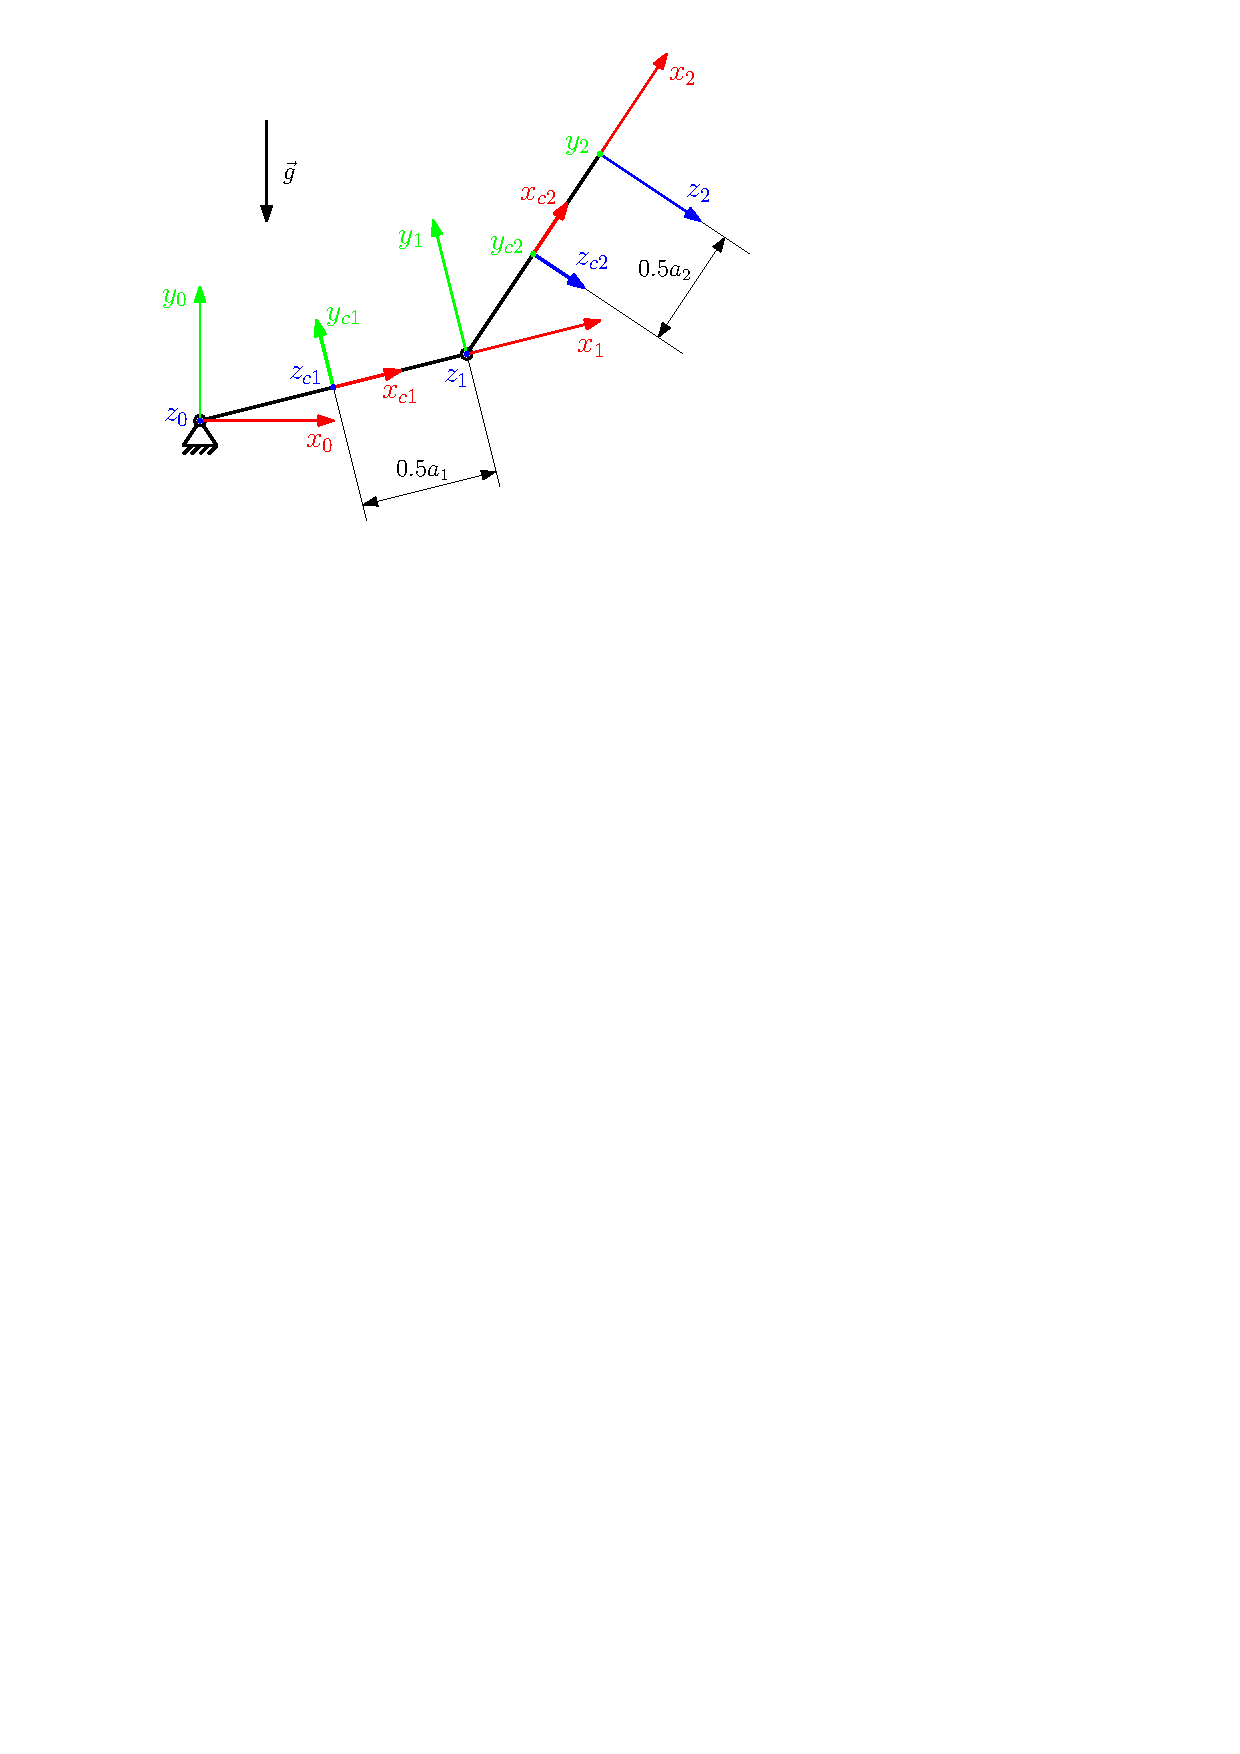
\includegraphics[width=0.95\linewidth]{manipulator_2_dynamics.pdf} \\ б)}
    \end{minipage}
    \caption{Схемы рассматриваемого манипулятора: а~--- кинематическая; б~--- демонстрирующая расположение барицентрических СК и СК КП.}
    \label{img_manipulator_2}
\end{figure}

Значения некоторых из динамических параметров звеньев:
\begin{gather}
    r^1_{1,\,c1} =
    \begin{bmatrix}
        -0.5 a_1 \\ 0 \\ 0
    \end{bmatrix}\!\!,
    \quad
    \mathcal{I}^{1}_1 =
    \begin{bmatrix}
        0 & 0 & 0 \\
        0 & \cfrac{m_1 a_1^2}{3} & 0 \\
        0 & 0 & \cfrac{m_1 a_1^2}{3}
    \end{bmatrix}\!\!,
    \\
    r^2_{2,\,c2} =
    \begin{bmatrix}
        -0.5 a_2 \\ 0 \\ 0
    \end{bmatrix}\!\!,
    \quad
    \mathcal{I}^{2}_2 =
    \begin{bmatrix}
        0 & 0 & 0 \\
        0 & \cfrac{m_2 a_2^2}{3} & 0 \\
        0 & 0 & \cfrac{m_2 a_2^2}{3}
    \end{bmatrix}\!\!\ldotp
\end{gather}

Параметры Денавита-Хартенберга, характеризующие взаимное расположение показанных на рисунке~\ref{img_manipulator_2} СК, приведены в таблице~\ref{table_DH_params_for_2}, где $\delta_1$ и $\delta_2$~--- некоторые константы.
Вектор ускорения свободного падения, выраженный в неподвижной СК равен
\begin{equation}
    g_0 =
    \begin{bmatrix}
        0 \\ -g \\ 0
    \end{bmatrix}\!\!\ldotp
\end{equation}

\begin{table}[h!]
    \caption{Параметры Денавита-Хартенберга}
    \begin{center}
        \begin{tabular}{|c|c|c|c|c|}
        \hline
        Звено, $i$ & $a_i$ & $\alpha_i$ & $d_i$ & $\theta_i$ \\
        \hline
        1 & $a_1$ & $0$ & $0$ & $\delta_1 - q_1$ \\
        \hline
        2 & $a_2$ & $\pi / 2$ & $0$ & $\delta_2 - q_2$ \\
        \hline
        \end{tabular}
    \end{center}
    \label{table_DH_params_for_2}
\end{table}

Матрицы однородных преобразований и проч.\footnote{В~пределах данного приложения принято следующее дополнительное обозначение:
\begin{equation*}
    \theta_{12} = \theta_1 + \theta_2 \ldotp
\end{equation*}
}:
\begin{align}
    & {}^0A_1 =
    \begin{bmatrix}
        c_1 & -s_1 & 0 & a_1 c_1 \\
        s_1 &  c_1 & 0 & a_1 s_1 \\
        0 & 0 & 1 & 0 \\
        0 & 0 & 0 & 1
    \end{bmatrix}\!\!,
    \quad
    {}^0R_1 =
    \begin{bmatrix}
        c_1 & -s_1 & 0 \\
        s_1 &  c_1 & 0 \\
        0 & 0 & 1
    \end{bmatrix}\!\!,
    \quad
    r^0_{0,\,1} =
    \begin{bmatrix}
        a_1 c_1 \\ a_1 s_1 \\ 0
    \end{bmatrix}\!\!,
    \\
    & {}^1A_2 =
    \begin{bmatrix}
        c_2 & 0 &  s_2 & a_2 c_2 \\
        s_2 & 0 & -c_2 & a_2 s_2 \\
        0 & 1 & 0 & 0 \\
        0 & 0 & 0 & 1
    \end{bmatrix}\!\!,
    \quad
    {}^1R_2 =
    \begin{bmatrix}
        c_2 & 0 &  s_2 \\
        s_2 & 0 & -c_2 \\
        0 & 1 & 0
    \end{bmatrix}\!\!,
    \quad
    r^0_{0,\,1} =
    \begin{bmatrix}
        a_2 c_2 \\ a_2 s_2 \\ 0
    \end{bmatrix}\!\!,
    \\
    & {}^0A_2 = {}^0A_1 {}^1A_2 =
    \begin{bmatrix}
        c_{12} & 0 &  s_{12} & a_2 c_{12} + a_1 c_1 \\
        s_{12} & 0 & -c_{12} & a_2 s_{12} + a_1 s_1\\
        0 & 1 & 0 & 1
    \end{bmatrix}\!\!,
    \quad
    {}^0R_2 =
    \begin{bmatrix}
        c_{12} & 0 &  s_{12} \\
        s_{12} & 0 & -c_{12} \\
        0 & 1 & 0
    \end{bmatrix}\!\!\ldotp
\end{align}
Иллюстрирующий правильность их расчета пример показан на рисунке~\ref{img_checking_example_for_2}.

\begin{figure}[h!]
    \centering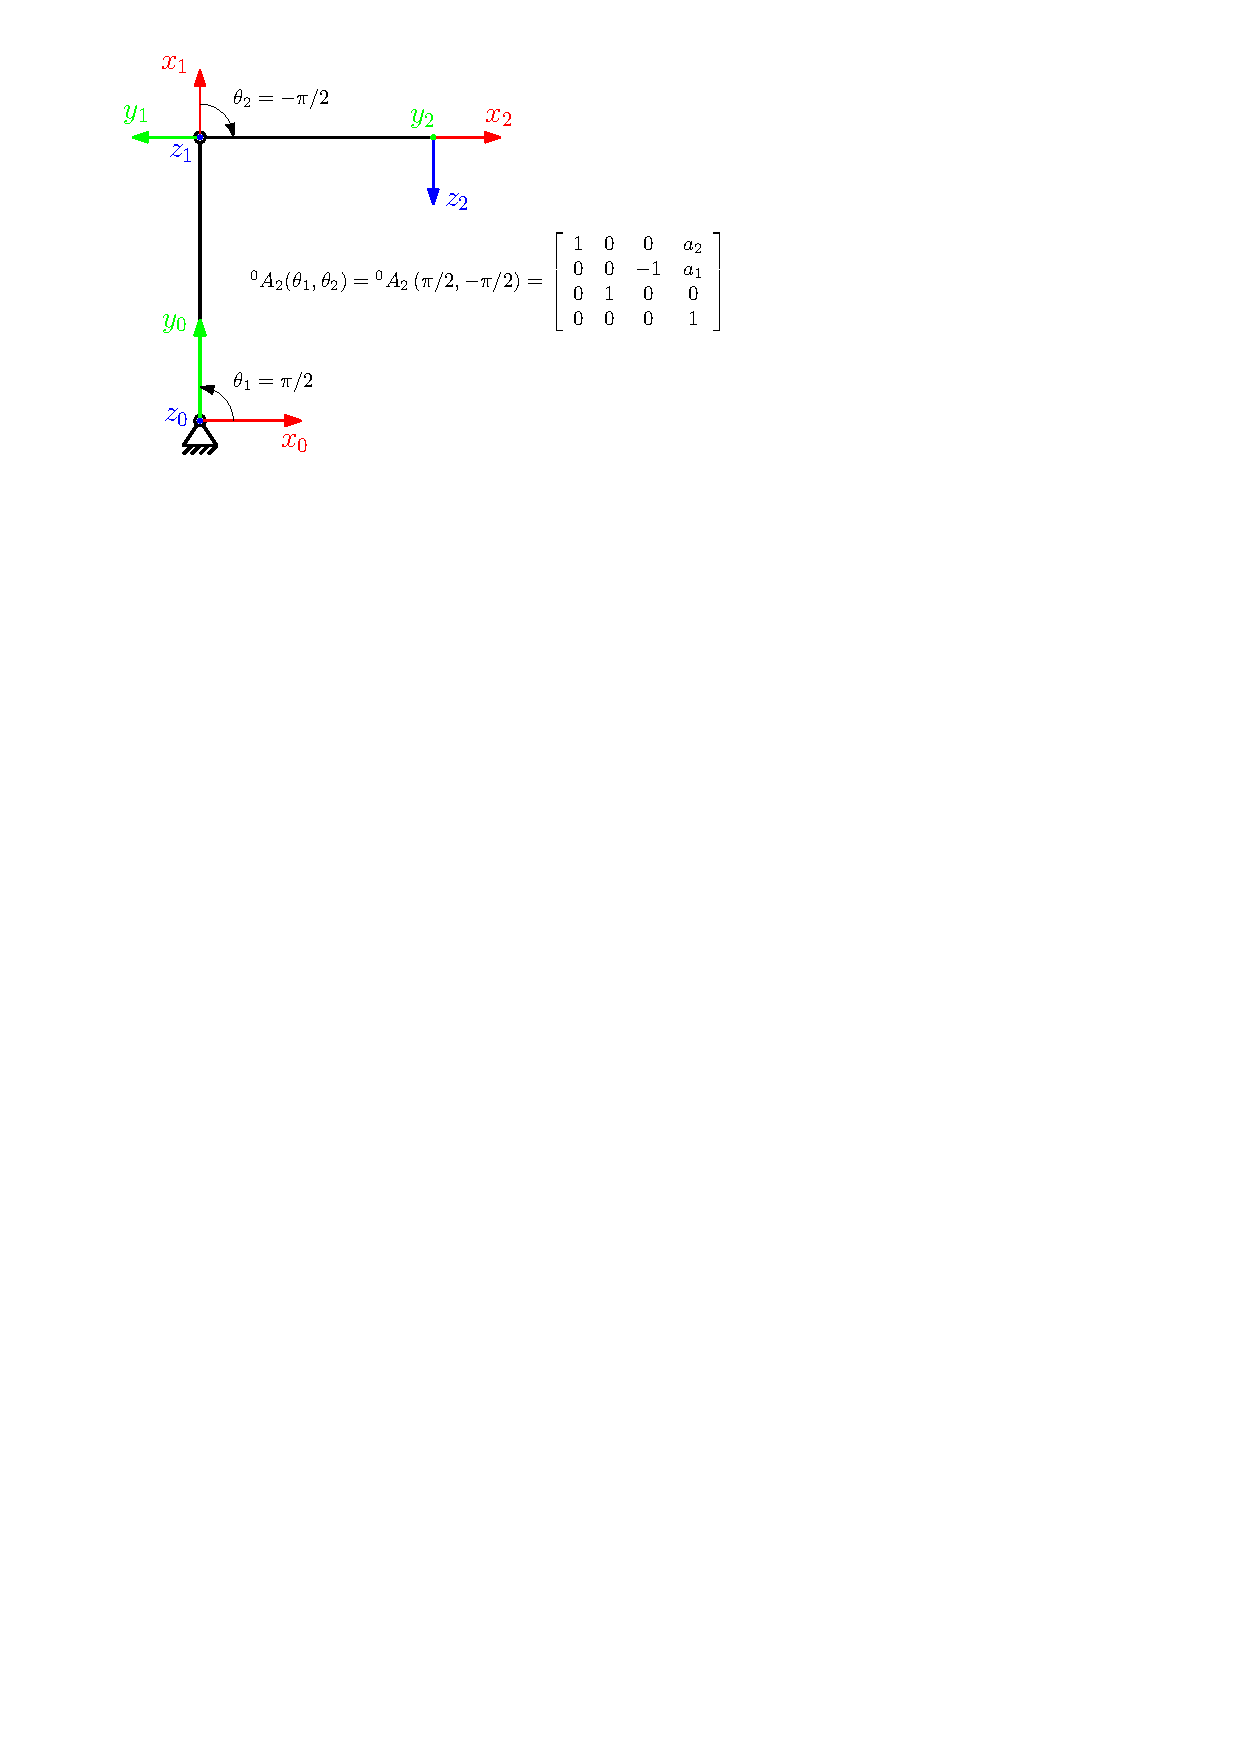
\includegraphics[width=0.65\textwidth]{checking_example_for_2.pdf}
    \vspace{0.2cm}
    \caption{Пример, проверяющий решение ПЗК для рассматриваемого манипулятора.}
    \label{img_checking_example_for_2}
\end{figure}

Некоторые подготовительные вычисления:
\begin{align}
    & r^1_{0,\,1} = {}^0R_1^T \!\cdot r^0_{0,\,1} =
    \begin{bmatrix}
        a_1 \\ 0 \\ 0
    \end{bmatrix}\!\!,
    \quad
    g_1 = {}^0R_1^T \!\cdot g_0 =
    \begin{bmatrix}
        -g s_1 \\ -g c_1 \\ 0
    \end{bmatrix}\!\!,
    \quad
    z^0_1 = {}^0R_1 \!\cdot z^1_1 =
    \begin{bmatrix}
        0 \\ 0 \\ 1
    \end{bmatrix}\!\!,
    \\
    & r^2_{0,\,2} = {}^0R_2^T \!\cdot r^0_{0,\,2} =
    \begin{bmatrix}
        a_2 + a_1 c_2 \\ 0 \\ a_1 s_2
    \end{bmatrix}\!\!,
    \quad
    g_2 = {}^0R_2^T \!\cdot g_0 =
    \begin{bmatrix}
        -g s_{12} \\ 0 \\ g c_{12}
    \end{bmatrix}\!\!\ldotp
    %
    \\[0.5cm]
    %
    & J_{v1} =
    \begin{bmatrix}
        z^0_0 \times (r^0_{0,\,1} - r^0_{0,\,0}) & \mathbf{0}
    \end{bmatrix}
    =
    \begin{bmatrix}
        -a_1 s_1 & 0 \\
        a_1 c_1 & 0 \\
        0 & 0
    \end{bmatrix}\!\!,
    \\
    & J_{v2} =
    \begin{bmatrix}
        z^0_0 \times (r^0_{0,\,2} - r^0_{0,\,0}) & z^0_1 \times (r^0_{0,\,2} - r^0_{0,\,1})
    \end{bmatrix}
    =
    \begin{bmatrix}
        -a_2 s_{12} - a_1 s_1 & -a_2 s_{12} \\
        a_2 c_{12} + a_1 c_1 & a_2 c_{12} \\
        0 & 0
    \end{bmatrix}\!\!,
    \\
    & J_{\omega1} =
    \begin{bmatrix}
        z^0_0 & \mathbf{0}
    \end{bmatrix}
    =
    \begin{bmatrix}
        0 & 0 \\
        0 & 0 \\
        1 & 0
    \end{bmatrix}\!\!,
    \qquad
    J_{\omega2} =
    \begin{bmatrix}
        z^0_0 & z^0_1
    \end{bmatrix}
    =
    \begin{bmatrix}
        0 & 0 \\
        0 & 0 \\
        1 & 1
    \end{bmatrix}\!\!\ldotp
\end{align}
\begin{align}
    & v^0_1 = -J_{v1} \dot{q} =
    \begin{bmatrix}
        a_1 s_1 \dot{q}_1 \\ -a_1 c_1 \dot{q}_1 \\ 0
    \end{bmatrix}\!\!, &
    \\
    & v^1_1 = {}^0R_1^T \!\cdot v^0_1 =
    \begin{bmatrix}
        0 \\ -a_1 \dot{q}_1 \\ 0
    \end{bmatrix}\!\!,
    \\
    &\omega^0_1 = -J_{\omega1} \dot{q} =
    \begin{bmatrix}
        0 \\ 0 \\ -\dot{q}_1
    \end{bmatrix}\!\!,
    \\
    & \omega^1_1 = {}^0R_1^T \!\cdot \omega^0_1 =
    \begin{bmatrix}
        0 \\ 0 \\ -\dot{q}_1
    \end{bmatrix}\!\!
    \\
    & v^0_2 = -J_{v2} \dot{q} =
    \begin{bmatrix}
        a_2 s_{12} (\dot{q}_1 + \dot{q}_2) + a_1 s_1 \dot{q}_1 \\
        -a_2 c_{12} (\dot{q}_1 + \dot{q}_2) - a_1 c_1 \dot{q}_1 \\
        0
    \end{bmatrix}\!\!,
    \\
    & v^2_2 = {}^0R_2^T \!\cdot v^0_2 =
    \begin{bmatrix}
        -a_1 s_2 \dot{q}_1 \\ 0 \\ a_2 (\dot{q}_1 + \dot{q}_2) + a_1 c_2 \dot{q}_1
    \end{bmatrix}\!\!,
    \\
    & \omega^0_2 = -J_{\omega2} \dot{q} =
    \begin{bmatrix}
        0 \\ 0 \\ -(\dot{q}_1 + \dot{q}_2)
    \end{bmatrix}\!\!,
    \\
    & \omega^2_2 = {}^0R_2^T \!\cdot \omega^0_2 =
    \begin{bmatrix}
        0 \\ -(\dot{q}_1 + \dot{q}_2) \\ 0
    \end{bmatrix}\!\!,
    \\
    & v^1_1 \times \omega^1_1 + g_1 =
    \begin{bmatrix}
        a_1 \dot{q}_1^2 - g s_1 \\ -g c_1 \\ 0
    \end{bmatrix}\!\!,
    \\
    & v^2_2 \times \omega^2_2 + g_2 =
    \begin{bmatrix}
    a_2 (\dot{q}_1 + \dot{q}_2)^2 + a_1 \dot{q}_1 (\dot{q}_1 + \dot{q}_2) c_2 - g s_{12} \\
    0 \\
    a_1 \dot{q}_1 (\dot{q}_1 + \dot{q}_2) s_2 + g c_{12}
    \end{bmatrix}\!\!\ldotp
\end{align}

Расчет составляющих функции Лагранжа:
\begin{align}
    & L_{1,1} = \frac{1}{2} (v^1_1)^T v^1_1 + g_1^T r^1_{0,\,1} = \frac{1}{2} a_1^2 \dot{q}_1^2 - a_1 g s_1,
    \\
    & L_{1,2} = x\{ v^1_1 \times \omega^1_1 + g_1 \} = a_1 \dot{q}_1^2 - g s_1,
    \\
    & L_{1,3} = y\{ v^1_1 \times \omega^1_1 + g_1 \} = -g c_1,
    \\
    & L_{1,4} = z\{ v^1_1 \times \omega^1_1 + g_1 \} = 0,
    \\
    & L_{1,5} = \frac{1}{2} \left( x\{ \omega^1_1 \} \right)^2 = 0,
    \\
    & L_{1,6} = \frac{1}{2} \left( y\{ \omega^1_1 \} \right)^2 = 0,
    \\
    & L_{1,7} = \frac{1}{2} \left( z\{ \omega^1_1 \} \right)^2 = \frac{1}{2} \dot{q}_1^2,
    \\
    & L_{1,8} = x\{ \omega^1_1 \} \cdot y\{ \omega^1_1 \} = 0,
    \\
    & L_{1,9} = x\{ \omega^1_1 \} \cdot z\{ \omega^1_1 \} = 0,
    \\
    & L_{1,10} = x\{ \omega^1_1 \} \cdot z\{ \omega^1_1 \} = 0,
    %
    \\[0.8cm]
    %
    & L_{2,1} = \frac{1}{2} (v^2_2)^T v^2_2 + g_2^T r^2_{0,\,2} = \frac{1}{2} (a_1 \dot{q}_1 s_2)^2 + \frac{1}{2} \bigl( a_2 (\dot{q}_1 + \dot{q}_2) + a_1 \dot{q}_1 c_2 \bigr)^2 - {}
    \\
    &\phantom{L_{2,1} = \frac{1}{2} (v^2_2)^T v^2_2 + g_2^T r^2_{0,\,2} =} {} - g s_{12}(a_2 + a_1 c_2) + a_1 g s_2 c_{12},
    \\
    & L_{2,2} = x\{ v^2_2 \times \omega^2_2 + g_2 \} = a_2 (\dot{q}_1 + \dot{q}_2)^2 + a_1 \dot{q}_1 (\dot{q}_1 + \dot{q}_2) c_2 - g s_{12},
    \\
    & L_{2,3} = y\{ v^2_2 \times \omega^2_2 + g_2 \} = 0,
    \\
    & L_{2,4} = z\{ v^2_2 \times \omega^2_2 + g_2 \} = a_1 \dot{q}_1 (\dot{q}_1 + \dot{q}_2) s_2 + g c_{12},
    \\
    & L_{2,5} = \frac{1}{2} \left( x\{ \omega^2_2 \} \right)^2 = 0,
    \\
    & L_{2,6} = \frac{1}{2} \left( y\{ \omega^2_2 \} \right)^2 = \frac{1}{2} (\dot{q}_1 + \dot{q}_2)^2,
    \\
    & L_{2,7} = \frac{1}{2} \left( z\{ \omega^2_2 \} \right)^2 = 0,
    \\
    & L_{2,8} = x\{ \omega^2_2 \} \cdot y\{ \omega^2_2 \} = 0,
    \\
    & L_{2,9} = x\{ \omega^2_2 \} \cdot z\{ \omega^2_2 \} = 0,
    \\
    & L_{2,10} = x\{ \omega^2_2 \} \cdot z\{ \omega^2_2 \} = 0 \ldotp
\end{align}

Расчет компонент регрессора:
\begin{align}
    & \mathcal{L}_1 \{ L_{1,1} \} = \frac{d}{dt}\frac{\partial L_{1,1}}{\partial\dot{q_1}} - \frac{\partial L_{1,1}}{\partial q_1} = a_1^2 \ddot{q}_1 - a_1 g c_1, \label{eq_first_regr_comp_for_2}
    \\
    & \mathcal{L}_1 \{ L_{1,2} \} = \frac{d}{dt}\frac{\partial L_{1,2}}{\partial\dot{q_1}} - \frac{\partial L_{1,2}}{\partial q_1} = 2 a_1 \ddot{q}_1 - g c_1,
    \\
    & \mathcal{L}_1 \{ L_{1,3} \} = g s_1,
    \\
    & \mathcal{L}_1 \{ L_{1,4} \} = 0,
    \\
    & \mathcal{L}_1 \{ L_{1,5} \} = 0,
    \\
    & \mathcal{L}_1 \{ L_{1,6} \} = 0,
    \\
    & \mathcal{L}_1 \{ L_{1,7} \} = \ddot{q}_1,
    \\
    & \mathcal{L}_1 \{ L_{1,8} \} = 0,
    \\
    & \mathcal{L}_1 \{ L_{1,9} \} = 0,
    \\
    & \mathcal{L}_1 \{ L_{1,10} \} = 0,
    %
    \\[0.8cm]
    %
    & \mathcal{L}_1 \{ L_{2,1} \} = \frac{d}{dt}\frac{\partial L_{2,1}}{\partial\dot{q_1}} - \frac{\partial L_{2,1}}{\partial q_1} = (a_1^2 + a_2^2 + 2 a_1 a_2 c_2) \ddot{q}_1 + (a_2^2 + a_1 a_2 c_2 )\ddot{q}_2 + {} \notag
    \\
    &\phantom{\mathcal{L}_1 \{ L_{2,1} \} =} + 2 a_1 a_2 \dot{q}_2 s_2 \dot{q}_1 + a_1 a_2 \dot{q}_2 s_2 \dot{q}_2 - a_2 g c_{12} - a_1 g c_1,
    \\
    & \mathcal{L}_1 \{ L_{2,2} \} = \frac{d}{dt}\frac{\partial L_{2,2}}{\partial\dot{q_1}} - \frac{\partial L_{2,2}}{\partial q_1} = 2 (a_2 + a_1 c_2) \ddot{q}_1 + (2 a_2 + a_1 c_2) \ddot{q}_2 + {} \notag
    \\
    &\phantom{\mathcal{L}_1 \{ L_{2,2} \} =} + 2 a_1 \dot{q}_2 s_2 \dot{q}_1 + a_1 \dot{q}_2 s_2 \dot{q}_2 - g c_{12},
    \\
    & \mathcal{L}_1 \{ L_{2,3} \} = 0,
    \\
    &\mathcal{L}_1 \{ L_{2,4} \} = 2 a_1 s_2 \ddot{q}_1 + a_1 s_2 \ddot{q}_2 - 2 a_1 \dot{q}_2 c_2 \dot{q}_1 - a_1 c_2 \dot{q}_2^2 - g s_{12},
    \\
    & \mathcal{L}_1 \{ L_{2,5} \} = 0,
    \\
    & \mathcal{L}_1 \{ L_{2,6} \} = \ddot{q}_1 + \ddot{q}_2,
    \\
    & \mathcal{L}_1 \{ L_{2,7} \} = 0,
    \\
    & \mathcal{L}_1 \{ L_{2,8} \} = 0,
    \\
    & \mathcal{L}_1 \{ L_{2,9} \} = 0,
    \\
    & \mathcal{L}_1 \{ L_{2,10} \} = 0,
\end{align}
\begin{align}
    &\mathcal{L}_2 \{ L_{2,1} \} = \frac{d}{dt}\frac{\partial L_{2,1}}{\partial\dot{q_2}} - \frac{\partial L_{2,1}}{\partial q_2} = (a_2^2 + a_1 a_2 c_2) \ddot{q}_1 +  a_2^2 \ddot{q}_2 - {} \notag
    \\
    &\phantom{\mathcal{L}_2 \{ L_{2,1} \} = \frac{d}{dt}\frac{\partial L_{2,1}}{\partial\dot{q_2}} - \frac{\partial L_{2,1}}{\partial q_2} =} - a_1 a_2 \dot{q}_1 s_2 \dot{q}_1 - a_2 g c_{12},
    \\
    & \mathcal{L}_2 \{ L_{2,2} \} = \frac{d}{dt}\frac{\partial L_{2,2}}{\partial\dot{q_2}} - \frac{\partial L_{2,2}}{\partial q_2} = (2 a_2 + a_1 c_2) \ddot{q}_1 + 2 a_2 \ddot{q}_2 - a_1 \dot{q}_1 s_2 \dot{q}_1 - g c_{12},
    \\
    & \mathcal{L}_2 \{ L_{2,3} \} = 0,
    \\
    & \mathcal{L}_2 \{ L_{2,4} \} = a_1 s_2 \ddot{q}_1 + a_1 \dot{q}_1 c_2 \dot{q}_1 - g s_{12},
    \\
    & \mathcal{L}_2 \{ L_{2,5} \} = 0,
    \\
    & \mathcal{L}_2 \{ L_{2,6} \} = \ddot{q}_1 + \ddot{q}_2,
    \\
    & \mathcal{L}_2 \{ L_{2,7} \} = 0,
    \\
    & \mathcal{L}_2 \{ L_{2,8} \} = 0,
    \\
    & \mathcal{L}_2 \{ L_{2,9} \} = 0,
    \\
    & \mathcal{L}_2 \{ L_{2,10} \} = 0 \ldotp \label{eq_last_regr_comp_for_2}
\end{align}

Уравнения движения робота c учетом~\eqref{eq_first_regr_comp_for_2}--\eqref{eq_last_regr_comp_for_2}:
\begin{align}
    & \left\{
    \begin{aligned}
        \!\!& m_1 \mathcal{L}_1 \{ L_{1,1} \} + m_1 x_{c1} \mathcal{L}_1 \{ L_{1,2} \} + m_1 y_{c1}  \mathcal{L}_1 \{ L_{1,3} \} + I_{1,\,zz} \mathcal{L}_1 \{ L_{1,7} \} + {} \\
        \!\!&{} + m_2 \mathcal{L}_1 \{ L_{2,1} \} + m_2 x_{c2} \mathcal{L}_1 \{ L_{2,2} \} + m_2 z_{c2}  \mathcal{L}_1 \{ L_{2,4} \} + I_{2,\,yy} \mathcal{L}_1 \{ L_{2,6} \} = \tau_1
        \\
        \!\!& m_2 \mathcal{L}_2 \{ L_{2,1} \} + m_2 x_{c2} \mathcal{L}_2 \{ L_{2,2} \} + m_2 z_{c2}  \mathcal{L}_2 \{ L_{2,4} \} + I_{2,\,yy} \mathcal{L}_2 \{ L_{2,6} \} = \tau_2
    \end{aligned}
    \right.
    \\[0.5cm]
    & \left\{
    \begin{aligned}
        \!\!& \bar{d}_{11} \ddot{q}_1 + \bar{d}_{12} \ddot{q}_2 + \bar{c}_{11} \dot{q}_1 + \bar{c}_{12} \dot{q}_2 + \bar{g}_{11} = \tau_1
        \\
        \!\!& \bar{d}_{21} \ddot{q}_1 + \bar{d}_{22} \ddot{q}_2 + \bar{c}_{21} \dot{q}_1 + \bar{c}_{22} \dot{q}_2 + \bar{g}_{21} = \tau_2
        \end{aligned}
    \right.
\end{align}
где
\begin{align}
    & \bar{d}_{11} = m_1 a_1^2 + 2 m_1 x_{c_1} a_1 + I_{1,\,zz} + m_2(a_1^2 + a_2^2 + 2 a_1 a_2 c_2) + {} \notag
    \\
    & \phantom{\bar{d}_{11} = } + 2 m_2 x_{c2} (a_2 + a_1 c_2) + 2 m_2 z_{c2} a_1 s_2 + I_{2,\,yy},
    \\
    & \bar{d}_{12} = m_2 (a_2^2 + a_1 a_2 c_2 ) + m_2 x_{c2} (2 a_2 + a_1 c_2) + m_2 z_{c2} a_1 s_2 + I_{2,\,yy},
    \\
    & \bar{d}_{21} = m_2(a_2^2 + a_1 a_2 c_2) + m_2 x_{c2} (2 a_2 + a_1 c_2) + m_2 z_{c2} a_1 s_2 + I_{2,\,yy},
    \\
    & \bar{d}_{22} = m_2 a_2^2 + 2 m_2 x_{c2} a_2 + I_{2,\,yy},
\end{align}
\begin{align}
    & \bar{c}_{11} = 2 m_2 a_1 a_2 \dot{q}_2 s_2 + 2 m_2 x_{c2} a_1 \dot{q}_2 s_2 - 2 m_2 z_{c2} a_1 \dot{q}_2 c_2,
    \\
    & \bar{c}_{12} = m_2 a_1 a_2 \dot{q}_2 s_2 + m_2 x_{c2} a_1 \dot{q}_2 s_2 - m_2 z_{c2} a_1 \dot{q}_2 c_2,
    \\
    & \bar{c}_{21} = -m_2 a_1 a_2 \dot{q}_1 s_2 - m_2 x_{c2} a_1 \dot{q}_1 s_2 + m_2 z_{c2} a_1 \dot{q}_1 c_2,
    \\
    & \bar{c}_{22} = 0,
    \\
    & \bar{g}_{11} = -m_1 a_1 g c_1 - m_1 x_{c1} g c_1 + m_1 y_{c1} g s_1 - m_2 (a_2 g c_{12} + a_1 g c_1) - {} \notag
    \\
    & \phantom{\bar{g}_{11} = } - m_2 x_{c2} g c_{12} - m_2 z_{c2} g s_{12},
    \\
    & \bar{g}_{21} = -m_2 a_2 g c_{12} - m_2 x_{c2} g c_{12}  - m_2 z_{c2} g s_{12} \ldotp
\end{align}

Матрицы $D(q)$, $C(q,\,\dot{q})$ и $G(q)$, с помощью которых они могут быть представлены в матричном виде равны
\begin{equation}\label{eq_matrices_from_first_example}
    D(q) =
    \begin{bmatrix}
        \bar{d}_{11} & \bar{d}_{12} \\
        \bar{d}_{21} & \bar{d}_{22}
    \end{bmatrix}\!\!,
    \qquad
    C(q,\,\dot{q}) =
    \begin{bmatrix}
        \bar{c}_{11} & \bar{c}_{12} \\
        \bar{c}_{21} & \bar{c}_{22}
    \end{bmatrix}\!\!,
    \qquad
    G(q) =
    \begin{bmatrix}
        \bar{g}_{11} \\ \bar{g}_{21}
    \end{bmatrix}\!\! \ldotp
\end{equation}

Пользуясь случаем можно убедиться в том, что формулы из раздела~\ref{part_matrix_form_of_equation} дают с дополнительным замечанием, о котором будет сказано ниже, такой же результат:
\begin{align}
    &J_{x1} =  - \bigl( J_{v1}^{\{3\}} \bigr)^T J_{\omega 1}^{\{2\}} + \bigl( J_{v1}^{\{2\}} \bigr)^T J_{\omega 1}^{\{3\}} =
    \begin{bmatrix}
        a_1 c_1 & 0 \\
        0 & 0
    \end{bmatrix}\!\!,
    \\
    &J_{y1} = \phantom{-}\bigl( J_{v1}^{\{3\}} \bigr)^T J_{\omega 1}^{\{1\}} - \bigl( J_{v1}^{\{1\}} \bigr)^T J_{\omega 1}^{\{3\}} =
    \begin{bmatrix}
        a_1 s_1 & 0 \\
        0 & 0
    \end{bmatrix}\!\!,
    \\
    &J_{z1} =  - \bigl( J_{v1}^{\{2\}} \bigr)^T J_{\omega 1}^{\{1\}} + \bigl( J_{v1}^{\{1\}} \bigr)^T J_{\omega 1}^{\{2\}} =
    \begin{bmatrix}
        0 & 0 \\
        0 & 0
    \end{bmatrix}\!\!,
    \\[0.5cm]
    &J_{x2} =  - \bigl( J_{v2}^{\{3\}} \bigr)^T J_{\omega 2}^{\{2\}} + \bigl( J_{v2}^{\{2\}} \bigr)^T J_{\omega 2}^{\{3\}} =
    \begin{bmatrix}
        a_2 c_{12} + a_1 c_1 & a_2 c_{12} + a_1 c_1 \\
        a_2 c_{12} & a_2 c_{12}
    \end{bmatrix}\!\!,
    \\
    &J_{y2} = \phantom{-}\bigl( J_{v2}^{\{3\}} \bigr)^T J_{\omega 2}^{\{1\}} - \bigl( J_{v2}^{\{1\}} \bigr)^T J_{\omega 2}^{\{3\}} =
    \begin{bmatrix}
        a_2 s_{12} + a_1 s_1 & a_2 s_{12} + a_1 s_1 \\
        a_2 s_{12} & a_2 s_{12}
    \end{bmatrix}\!\!,
    \\
    &J_{z2} =  - \bigl( J_{v2}^{\{2\}} \bigr)^T J_{\omega 2}^{\{1\}} + \bigl( J_{v2}^{\{1\}} \bigr)^T J_{\omega 2}^{\{2\}} =
    \begin{bmatrix}
        0 & 0 \\
        0 & 0
    \end{bmatrix}\!\!,
\end{align}
\begin{align}
    & r^0_{1,\,c1} = {}^0\!R_1 r^1_{1,\,c1} =
    \begin{bmatrix}
        x_{c1} c_1 - y_{c1} s_1 \\
        x_{c1} s_1 + y_{c1} c_1 \\
        z_{c1}
    \end{bmatrix}\!\!,
    \quad
    r^0_{2,\,c2} = {}^0\!R_2 r^2_{2,\,c2} =
    \begin{bmatrix}
        x_{c2} c_{12} + z_{c2} s_{12} \\
        x_{c2} s_{12} + z_{c2} c_{12} \\
        y_{c2}
    \end{bmatrix}\!\!,
    \\[0.5cm]
     & \mathcal{D}(q) = \sum_{i=1}^2 \Bigl(m_i J_{vi}^T J_{vi} + J_{\omega i}^T \, {}^0\!R_i \, \mathcal{I}^{i}_i \, {}^0\!R_i^T J_{\omega i} + 2 \cdot x\{ m_i r^0_{i,\,ci} \} \!\cdot\! J_{xi} + {}
     \\
     & \phantom{\mathcal{D}(q) = \sum_{i=1}^2 \Bigl(} +  2 \cdot y\{ m_i r^0_{i,\,ci} \} \!\cdot\! J_{yi} + 2 \cdot z\{ m_i r^0_{i,\,ci} \} \!\cdot\! J_{zi}\Bigr) =
     \begin{bmatrix}
         \mathcal{D}_{11} & \mathcal{D}_{12} \\
         \mathcal{D}_{21} & \mathcal{D}_{22} \\
     \end{bmatrix}\!\!,
    \\[0.5cm]
    & D(q) =
    \begin{bmatrix}
        \mathcal{D}_{11} & 0.5 ( \mathcal{D}_{12} + \mathcal{D}_{21} ) \\
        0.5 ( \mathcal{D}_{12} + \mathcal{D}_{21} ) & \mathcal{D}_{22}
    \end{bmatrix}
    =
    \begin{bmatrix}
        D_{11} & D_{12} \\
        D_{21} & D_{22}
    \end{bmatrix}\!\!,
\end{align}
где
\begin{align}
    & \mathcal{D}_{11} = \bar{d}_{11},
    \\
    & \mathcal{D}_{12} = 2 m_2 a_1 s_2  z_{c2} + (2 m_2 a_2 + 2 m_2 a_1 c_2) x_{c2} + m_2 a_1 a_2 c_2 + m_2 a_2^2 + I_{2,\,yy},
    \\
    & \mathcal{D}_{21} = 2 m_2 a_2 x_{c2} + m_2 a_1 a_2 c_2 + m_2 a_2^2 + I_{2,\,yy},
    \\
    & \mathcal{D}_{22} = \bar{d}_{22},
    \\
    & D_{11} = \mathcal{D}_{11},
    \\
    & D_{12} = \bar{d}_{12}
    \\
    & D_{21} = D_{12},
    \\
    & D_{22} = \mathcal{D}_{22},
    \\[0.5cm]
    & C_{111} = \frac{1}{2} \left( \frac{\partial D_{11}}{\partial q_1} + \frac{\partial D_{11}}{\partial q_1} - \frac{\partial D_{11}}{\partial q_1} \right) = 0,
    \\
    & C_{112} = \frac{1}{2} \left( \frac{\partial D_{21}}{\partial q_1} + \frac{\partial D_{21}}{\partial q_1} - \frac{\partial D_{11}}{\partial q_2} \right) = m_2 a_1 (c_2 z_{c2} - s_2 x_{c2} - a_2 s_2),
    \\
    & C_{121} = \frac{1}{2} \left( \frac{\partial D_{12}}{\partial q_1} + \frac{\partial D_{11}}{\partial q_2} - \frac{\partial D_{12}}{\partial q_2} \right) = m_2 a_1 (s_2 x_{c2} - c_2 z_{c2} + a_2 s_2),
    \\
    & C_{122} = \frac{1}{2} \left( \frac{\partial D_{22}}{\partial q_1} + \frac{\partial D_{21}}{\partial q_2} - \frac{\partial D_{12}}{\partial q_2} \right) = 0,
\end{align}
\begin{align}
    & C_{211} = \frac{1}{2} \left( \frac{\partial D_{11}}{\partial q_2} + \frac{\partial D_{12}}{\partial q_1} - \frac{\partial D_{21}}{\partial q_1} \right) = m_2 a_1 (s_2 x_{c2} - c_2 z_{c2} + a_2 s_2),
    \\
    & C_{212} = \frac{1}{2} \left( \frac{\partial D_{21}}{\partial q_2} + \frac{\partial D_{22}}{\partial q_1} - \frac{\partial D_{21}}{\partial q_2} \right) = 0,
    \\
    & C_{221} = \frac{1}{2} \left( \frac{\partial D_{12}}{\partial q_2} + \frac{\partial D_{12}}{\partial q_2} - \frac{\partial D_{22}}{\partial q_1} \right) = m_2 a_1 (s_2 x_{c2} - c_2 z_{c2} + a_2 s_2),
    \\
    & C_{222} = \frac{1}{2} \left( \frac{\partial D_{22}}{\partial q_2} + \frac{\partial D_{22}}{\partial q_2} - \frac{\partial D_{22}}{\partial q_2} \right) = 0,
    \\[0.5cm]
    & C_{11} = C_{111} \dot{q}_1 + C_{211} \dot{q}_2 = m_2 a_1 \dot{q}_2 ( x_{c2} s_2 - z_{c2}c_2 + a_2 s_2),
    \\
    & C_{12} = C_{121} \dot{q}_1 + C_{221} \dot{q}_2 = m_2 a_1 (\dot{q}_1 + \dot{q}_2) (x_{c2} s_2 - z_{c2} c_2 + a_2 s_2),
    \\
    & C_{21} = C_{112} \dot{q}_1 + C_{212} \dot{q}_2 = -m_2 a_1 \dot{q}_1 ( x_{c2} s_2 - z_{c2}c_2 + a_2 s_2),
    \\
    & C_{22} = C_{122} \dot{q}_1 + C_{222} \dot{q}_2 = 0,
    \\[0.5cm]
    & C(q,\,\dot{q}) =
    \begin{bmatrix}
        C_{11} & C_{12} \\
        C_{21} & C_{22}
    \end{bmatrix}\!\!, \label{eq_second_c_in_first_example}
    \\[0.3cm]
    &U = -\sum_{i=1}^2 \left( m_i g_i^T r^i_{0,\,i} + g_i^T (m_ir^i_{i,\,ci}) \right) = - m_2 g c_{12} z_{c2} + m_1 g c_1 y_{c1} + {}
    \\
    &\phantom{U =} + m_2 g s_{12} x_{c2} + m_1 g s_1 x_{c1} + m_2 g a_2 s_{12} + m_2 a_1 g s_1 + m_1 a_1 g s_1,
    \\[0.3cm]
    &\begin{aligned}
    & G_{11} = \frac{\partial U}{\partial q_1} = \bar{g}_{11},
    \\
    & G_{21} = \frac{\partial U}{\partial q_2} = \bar{g}_{21},
    \end{aligned}
    \qquad \Rightarrow \qquad
    G(q) =
    \begin{bmatrix}
        G_{11} \\ G_{21}
    \end{bmatrix}\!\!\ldotp
\end{align}
Нетрудно видеть, что выражение, полученное таким образом для~$C(q,\,\dot{q})$ не совпадает с ее версией из~\eqref{eq_matrices_from_first_example}.
Это не является ошибкой, а происходит из-за того, что данная матрица может иметь несколько вариантов представления.
В~такой ситуации, главное, чтобы последние давали один и тот же результат при подстановке в выражение $C(q,\,\dot{q}) \cdot \dot{q}$.
Это и будет являться критерием их равнозначности.
Для версий матрицы $C(q,\,\dot{q})$ из~\eqref{eq_matrices_from_first_example} и~\eqref{eq_second_c_in_first_example} оно имеет следующее значение:
\begin{equation}
    C(q,\,\dot{q}) \cdot \dot{q} =
    \begin{bmatrix}
        m_2 a_1 (2 \dot{q}_1 \dot{q}_2 + \dot{q}_2^2) \bigl( s_2 x_{c2} - c_2 z_{c2} + a_2 s_2 \bigr) \\
        m_2 a_1 \dot{q}_1^2 (c_2 z_{c2} - s_2 x_{c2} - a_2 s_2)
    \end{bmatrix}\!\!\ldotp
\end{equation}
